\documentclass[12pt,twoside]{tesis}
% Formato Latex para Tesis de Doctorado Universidad Nacional del Sur, (c) 2000 Alejandro J. Garc�a
% Solamente se sabe lo que significa escribir una tesis, cuando se ha terminado de escribir una.
% Espero que estos archivos sean de utilidad y ahorren bastante tiempo al que lo use. Ale.

\usepackage{a4}
\usepackage{t_encab}
\usepackage{latexsym}
\usepackage{amsthm}
\usepackage{epstopdf}
\usepackage{enumerate}
\usepackage{tikz}
\usepackage[spanish]{babel}
\usepackage[latin1]{inputenc}
%\usepackage[pdftex]{graphicx}

\selectlanguage{spanish}

% Definicion de los encabezamientos de t_encab.sty
\pagestyle{fancyplain}
\lhead[\fancyplain{}{\normalsize\thepage}]
{\fancyplain{}{\normalsize\rightmark}}
\rhead[\fancyplain{}{\normalsize\leftmark}]
{\fancyplain{}{\normalsize\thepage}}
\chead{}\lfoot{}\rfoot{}\cfoot{}

\newcommand{\clearemptydoublepage}{\newpage\thispagestyle{empty}\cleardoublepage}

\theoremstyle{definition}
\newtheorem{definicion}{Definición}[section]
\theoremstyle{example}
\newtheorem{ejemplo}{Ejemplo}[section]

\newcommand{\ie        }{i.\,e.}
\newcommand{\etal      }{\mbox{{\em et al.}}}
\newcommand{\eg        }{e.\,g.}
\newcommand{\raya      }{\rule{\textwidth}{.05mm}}
\newcommand{\eoe       }{\begin{flushright}$\Box$\end{flushright}}
\newcommand{\marginnote}[1]{\marginpar{\frame{#1}}}
\newcommand{\new       }{\marginpar{\frame{\sc new}}}

\newcommand{\DLP     }{\mbox{DeLP}}
\newcommand{\DLPa    }{\mbox{DeLP}}
\newcommand{\DLPas   }{\mbox{DeLP(a)-strict}}
\newcommand{\DLPans  }{\mbox{DeLP(a)-non-strict}}
\newcommand{\dlp     }{\mbox{\it de.l.p.}}
\newcommand{\cree    }{B}
\newcommand{\no      }{\mbox{$\sim$}}
\newcommand{\negda   }[1]{\mbox{\textsf{not}$#1$}}
\newcommand{\naf     }{\p{$\backslash$+}}
\newcommand{\notj    }{{not}}
\newcommand{\comp    }[1]{\mbox{$\overline{#1}$}}
\newcommand{\simbcomp}{ $\stackrel{\comp{\ \ }}{\vrule width 0pt height.8ex}$ }
\newcommand{\p       }[1]{{\small \tt #1}}

% DLP programs 
% strict rule
\newcommand{\srule}[2]{\mbox{$ #1\;\leftarrow\;#2$}}
%\newcommand{\fact}[1]{\mbox{$ #1$}}  % some cls files have \fact defined for other things 
\newcommand{\facto}[1]{\mbox{$ #1$}} % for compatibility when the reason above holds
% literal
\newcommand{\lit}[1]{\mbox{$ #1$}}
% defesible rule
\newcommand{\drule}[2]{\mbox{$ #1\; \defleftarrow \; #2$}}
\newcommand{\defleftarrow}{{\raise1.5pt\hbox{\tiny\defleft}}}
\newcommand{\defleft}{\mbox{---\hspace{-1.5pt}\raise.05pt\hbox{$<$}}}
% presumption
%\newcommand{\presum}[1]{\drule{#1}{true}}
\newcommand{\presum}[1]{\drule{#1}{}}
% inverted rules
\newcommand{\invleftarrow}{ $\hookleftarrow $ }
\newcommand{\irule}[2]{\mbox{$#1$ \invleftarrow $#2$}}
\newcommand{\dquery}[1]{\drule{}{#1}}

% Donald Nute rules
\newcommand{\rr}[2]{\mbox{$ #1 \Rightarrow #2 $}} % defeasible
\newcommand{\re}[2]{\mbox{$#1 \rightarrow #2 $}} % strict
\newcommand{\de}[2]{\mbox{$ #1 \leadsto #2$}} %defeater

% Programcion en Logica Extendida
\newcommand{\ple}{\mbox{\sc PLE}}
\newcommand{\extclause}[2]{\mbox{ #1 $\leftarrow$ #2}}
\newcommand{\true}{$true$}

% flecha rebatible para la derecha
\newcommand{\defrightarrow}{\mbox{$\succ\!$---}}
\newcommand{\defarrow}{{\raise1.5pt\hbox{\tiny\defrightarrow}}}

% Argumentos
\newcommand{\ArgA}{\mbox{${\mathcal A}$}}
\newcommand{\Ap}{\mbox{\ArgA$'$}}
\newcommand{\ArgAo}{\mbox{${\mathcal A_0}$}}
\newcommand{\ArgAa}{\mbox{${\mathcal A_1}$}}
\newcommand{\ArgAb}{\mbox{${\mathcal A_2}$}}
\newcommand{\ArgAn}{\mbox{${\mathcal A_n}$}}
\newcommand{\ArgAi}{\mbox{${\mathcal A_i}$}}
\newcommand{\ArgAim}{\mbox{${\mathcal A_{i-1}}$}}
\newcommand{\ArgB}{\mbox{${\mathcal B}$}}
\newcommand{\ArgBo}{\mbox{${\mathcal B_0}$}}
\newcommand{\ArgBa}{\mbox{${\mathcal B_1}$}}
\newcommand{\ArgBb}{\mbox{${\mathcal B_2}$}}
\newcommand{\ArgBk}{\mbox{${\mathcal B_k}$}}
\newcommand{\ArgQ}{\mbox{${\mathcal Q}$}}
\newcommand{\ArgQo}{\mbox{${\mathcal Q_0}$}}
\newcommand{\ArgQa}{\mbox{${\mathcal Q_1}$}}
\newcommand{\ArgQb}{\mbox{${\mathcal Q_2}$}}
\newcommand{\ArgQk}{\mbox{${\mathcal Q_k}$}}
\newcommand{\ArgQn}{\mbox{${\mathcal Q_n}$}}
\newcommand{\ArgQi}{\mbox{${\mathcal Q_i}$}}
\newcommand{\ArgQim}{\mbox{${\mathcal Q_{i-1}}$}}
\newcommand{\AQ}{\mbox{$\langle \ArgA,\ArgQ \rangle $}}
\newcommand{\AoQo}{\mbox{$\langle \ArgAo,\ArgQo \rangle $}}
\newcommand{\AaQa}{\mbox{$\langle \ArgAa,\ArgQa \rangle $}}
\newcommand{\AbQb}{\mbox{$\langle \ArgAb,\ArgQb \rangle $}}
\newcommand{\AnQn}{\mbox{$\langle \ArgAn,\ArgQn \rangle $}}
\newcommand{\AiQi}{\mbox{$\langle \ArgAi,\ArgQi \rangle $}}
\newcommand{\AimQim}{\mbox{$\langle \ArgAim,\ArgQim \rangle $}}
\newcommand{\BaQa}{\mbox{$\langle \ArgBa,\ArgQa \rangle $}}
\newcommand{\BkQk}{\mbox{$\langle \ArgBk,\ArgQk \rangle $}}
\newcommand{\Argum}[2]{\mbox{$\langle #1, #2 \rangle $}}
\newcommand{\AS}[2]{$\langle \{#1\}, #2 \rangle $}
\newcommand{\bigAS}[2]{$\bigl\langle \{#1\}, #2 \bigr\rangle $}
\newcommand{\nlA}[1]{$$\mbox{#1}$$}

% Sets of rules
\newcommand{\Facts}{\mbox{$\Theta$}}                            % Facts
\newcommand{\SRules}{\mbox{$\Omega$}}                           % Stricts rules
\newcommand{\SSet}{\mbox{$\Pi$}}                                % Stricts rules & facts
\newcommand{\SSg}{\mbox{${\SSet}_G$}}                           % Stricts rules without facts 
\newcommand{\SSp}{\mbox{${\SSet}_P$}}                           % set of facts
\newcommand{\DD}{\mbox{$\Delta$}}                               % Defeasible rules
\newcommand{\SD}{\mbox{$(\SSet,\DD)$}}                          % sets of rules of a program 
\newcommand{\FSD}{\mbox{$(\Facts,\SRules,\DD)$}}                % sets of rules of a program 
\newcommand{\Presumptions}{\mbox{$\Phi$}}                       % 
\newcommand{\DDp}{\mbox{$\Delta^{+}$}}                          % Defeasible rules and presumptions
\newcommand{\SDp}{\mbox{$(\SSet,\DDp)$}}                        % sets of rules of a program 
\newcommand{\FSDP}{\mbox{$(\Facts,\SRules,\DD,\Presumptions)$}} % sets of rules of a program 

\newcommand{\FySyD}{\mbox{\Facts\ $\cup$ \SSet\ $\cup$ \DD}}   
\newcommand{\SyD}{\mbox{\SSet\ $\cup$ \DD}}   
\newcommand{\SyA}{\mbox{\SSet\ $\cup$ \ArgA}}
\newcommand{\SyAp}{\mbox{\SSet\ $\cup$ \Ap}}
\newcommand{\SyArga}{\mbox{\SSet\ $\cup$ \Arga}}
\newcommand{\RR}{\mbox{$\mathcal R$}}
\newcommand{\PP}{\mbox{${\mathcal P}$}}
\newcommand{\PPa}{\mbox{${\mathcal P}_1$}}
\newcommand{\PPb}{\mbox{${\mathcal P}_2$}}
\newcommand{\PPc}{\mbox{${\mathcal P}_3$}}
\newcommand{\PPd}{\mbox{${\mathcal P}_4$}}
\newcommand{\FFi}{\mbox{${\mathcal F}_i$}}
\newcommand{\FF}{\mbox{${\mathcal F}$}}

\newcommand{\SyQaQ}{\mbox{$\SSet \cup \{\ArgQa\\,\ArgQ\}$}}

\begin{document}

\pagestyle{empty}

%
\vspace{3cm}

%\input setbmp

\begin{center}
\thispagestyle{empty}

\

\

\

\

\hspace{-5cm} % para dvi
%\hspace{-3cm} % para ps
\special{bmp: uni.bmp x=2 y=2}

%\centerbmp{5cm}{5cm}{c:uni.bmp}

\

{\Large {\sc Universidad Nacional del Sur}}\\

\

\

{\Large {\sc Tesina de Grado en Ciencias de la Computaci\'on}}\\


\

\

{\Large {\bf Titulo de la Tesina:}}\\ 
\vspace{2mm}
{\Large {\bf Subtitulo de la Tesina}} \\
\vspace{1mm}
{\Large {\bf Palabra suelta del subtitulo}}

\

\

\

{\Large I\~{n}aki Garay}\\
\vspace{4cm}
{\Large {\sc Bah\'\i a Blanca}\hspace{6cm}{\sc Argentina}}\\
\ \\
{\Large 2013}\ 

\end{center}

\break
   
%\clearemptydoublepage

%% \chapter*{Prefacio}
% 
% Esta Tesis es presentada como parte de los requisitos para optar
% al grado acad\'emico de Doctor en Ciencias de la Computaci\'on,
% de la Universidad Nacional del Sur, y no ha sido presentada previamente
% para la obtenci\'on de otro t\'{\i}tulo en esta Universidad u otras.
% La misma contiene los resultados obtenidos en
% investigaciones llevadas a cabo en el
% Departamento de Ciencias de la Computaci\'on, 
% durante el per\'\i odo comprendido entre 
% el 1 de noviembre de 1997 y el 10 de noviembre de 2000, 
% bajo la direcci\'on del Dr. Guillermo R. Simari, Profesor
% Titular del Departamento de Ciencias de la Computaci\'on.

\vspace{5cm}

\begin{flushright}
I\~{n}aki Garay \\
{\small \tt igarai@gmail.com} \\
{\sc Departamento de Ciencias de la Computaci\'on \\
Universidad Nacional del Sur }\\
Bah\'{\i}a Blanca, Octubre de 2012. \\
\end{flushright}
 
%\clearemptydoublepage

%Padre, Esposa, Madre, Novia, Amigos 
%\clearemptydoublepage

\pagenumbering{roman} 
\setcounter{page}{1}

\tableofcontents 
\clearemptydoublepage

\pagestyle{fancyplain}
\pagenumbering{arabic} 
\setcounter{page}{1}

%\chapter{Introducción}
\label{chap:introduccion}

\begin{quote}
\scriptsize{
    \emph{
        If your thesis is utterly vacuous   \\
        Use first-order predicate calculus  \\
            With sufficient formality       \\
            The sheerest banality           \\
        Will be hailed by the critics:      \\
            ``Miraculous''                  \\
        }
    - Henry Kautz
}
\end{quote}

\section{Enunciado}
  \label{sec:enunciado}

  El objetivo de este trabajo es presentar en detalle el sistema de
  comunicación de percepciones entre agentes utilizado en el sistema
  multi-agente desarrollado en el marco de MAPC 2011\footnote{Multi-
  Agent Programming Contest 2011 - http://www.multiagentcontest.org/},
  la representación de la base de conocimiento utilizada, las decisiones
  de diseño e implementación tomadas, aspectos exitosos y las
  posibilidades de mejora.
  
  En esta instancia de la competencia se hizo énfasis en lograr un
  Sistema Multi-Agente puramente distribuido en el cual cada agente
  realiza un proceso de toma de decisiones independiente en lugar de
  contar con una inteligencia centralizada que decide cuál será la
  acción a realizar para cada uno de los agentes. 
  
  Para asegurar que las decisiones de cada agente sean lo mas informadas
  posibles, se desarrolló un sistema de sincronización de la base de
  conocimiento que opera en una fase previa al proceso deliberativo de
  cada agente, asegurando que todos los agentes sepan lo mismo sobre el
  estado actual del mundo.
  
  El objetivo particular de este proyecto es la aplicación de
  Argumentación para la implementación de diálogos entre agentes
  inmersos en un escenario con objetivos determinados.
  Puntualmente, se enfocará la investigación a la plataforma propuesta
  en el Multi-Agent Programming Contest, un juego académico donde
  agentes independientes compiten por diferentes objetivos.
  Sin embargo, el desarrollo de herramientas para implementar tales
  formalismos se encuentra en progreso y a un paso más lento.
  Además, muchas de las herramientas disponibles carecen de una base
  formal y suelen ser simplemente un entorno de desarrollo amigable.

\section{Organización del trabajo}
  \label{sec:organizacion_del_trabajo}
  
  El capítulo \ref{chap:definiciones_preliminares} da un conjunto de
  definiciones y un marco teórico sobre el cual se trabajó, abarcando
  los conceptos de agentes, arquitectura BDI, programacion lógica
  rebatible, y el contexto de desarrollo
  
  El capítulo \ref{chap:arquitectura} describe la arquitectura general e
  interna de cada agente, incluyendo la entrada y salida de datos, las
  fases de preprocesamiento de las percepciones, el esquema de
  representacion de conocimiento utilizada y el proceso deliberativo
  realizado por cada agente.
  
  El capítulo \ref{chap:servidor_de_percepciones} describe en detalle el
  sistema de sincronizacion de la base de conocimientos de cada agente,
  su funcionamiento interno, capacidades y limitaciones.
  
 
%\clearemptydoublepage

%% Contexto de la tesis (background formal, y contexto del desarrollo

\chapter{Definiciones preliminares} 
\label{chap:definiciones_preliminares}

En este capítulo se revisarán algunas definiciones de conceptos
técnicos, para posteriormente utilizarlos sin ambigüedad durante el
resto de la presentación.

\section{Agente inteligente}
\label{sec:agente_inteligente}

Un agente es una entidad computacional autónoma, que puede percibir su
entorno a través de sensores, y actuar en dicho entorno utilizando
efectores.
Usualmente, la información que un agente percibe de su entorno es sólo
parcial.
Los agentes toman decisiones a partir de la información contenida en
su base de conocimiento, siguiendo diferentes conjuntos de reglas
propuestas, y actúan de manera acorde a la decisión tomada.
Dichas acciones, a su vez, pueden producir efectos en el entorno.

Actualmente los agentes tienen un campo de aplicación muy amplio y
existen muchos tipos de agentes diferentes (por ejemplo:
\textit{reactivos}, \textit{deliberativos}, \textit{inteligentes},
\textit{de interface}, \textit{colaborativos}), los cuales a su vez
están orientados a distintos entornos de aplicación.

En la mayoría de los casos, los agentes no existen por sí solos, sino
que participan de un Sistema Multi-Agente (SMA).

\section{Sistema Multi-Agente}
\label{sec:sistema_multiagente}

En un Sistema Multi-Agente (SMA) mas de un agente interactúan para
lograr un objetivo o realizar una tarea común.
Cada agente tiene información incompleta y capacidades limitadas, el
control del sistema es distribuido, los datos están descentralizados,
y la computación es asincrónica.
Los agentes se desenvuelven en un entorno dinámico y cambiante, el
cual no puede predecirse y se ve afectado por las acciones que son
llevadas a cabo.

Un aspecto importante en SMA es la comunicación entre agentes, la cual
puede ser necesaria para que los agentes compitan o cooperen de
acuerdo a sus metas individuales. 
Los diálogos con otros agentes del mismo ambiente son, actualmente, un
área de estudio intensivo.
 
%
\section{Modelo BDI}
 \label{sec:modelo_bdi}
 
 % El \textit{modelo Creencia-Deseo-Intención}, en adelante \textit{BDI}
 % (\textit{Belief-Desire-Intention}), es un modelo desarrollado para el
 % diseño de agentes inteligentes, basado en una vista simplificada de la
 % inteligencia humana.
 % Como se analizará en la sección \ref{sec:arquitectura_bdi}, el sistema
 % presentado en este trabajo implementa una  adaptación de dicho modelo.
 % Por esta razón, se introducen en esta sección los  conceptos básicos
 % relacionados, que sirvieron de base para nuestro desarrollo.
 
 
 % El modelo BDI está dedicado al modelado formal del razonamiento
 % práctico, es  decir, la formalización de las bases y explicaciones
 % psicológicas y filosóficas  (provenientes principalmente de la
 % filosofía de la mente y de la acción) de los  conceptos de agente,
 % acción, intención, creencia, voluntad, deliberación,  razonamiento de
 % medios y fines, etc.
 % El razonamiento práctico es incorporado  en agentes (por ejemplo, los
 % seres humanos) capaces de perseguir y, por lo tanto,  comprometerse
 % con una determinada meta factible (una acción en particular)  a través
 % de una cuidadosa planificación de los medios, de las condiciones
 % previas  y las acciones que conducen a ese objetivo.


 % Estos conceptos son incorporados al modelo mediante la implementación
 % de los  aspectos principales de la teoría del razonamiento práctico
 % humano de Michael Bratman (también referido como Belief-Desire-
 % Intention, o BDI).
 % Es decir, implementa  las nociones de creencia, deseo y (en
 % particular) intención, de una manera inspirada  por Bratman.
 % Una discusión más extensa puede ser encontrada en el mencionado
 % trabajo de Bratman\cite{brat99} y Searle\cite{searle1985}.
 
 
 % Este basamento teórico permite al modelo resolver un problema
 % particular que  se presenta en la programación de agentes.
 % Provee un mecanismo para separar la  actividad de seleccionar un plan
 % de la ejecución de los planes actualmente activos.
 % Los agentes BDI son capaces de balancear el tiempo invertido en
 % deliberar sobre los planes (elegir qué hacer) y ejecutar estos planes
 % (llevarlo a cabo).
 % La actividad  de crear los planes en primera instancia, escapa al
 % alcance del modelo.

\subsection{Creencias, Deseos e Intenciones}
 \label{sec:creencia_deseos_intenciones}
 
 % Las \textit{creencias, deseos e intenciones} son consideradas estados
 % mentales  intencionales (de forma opuesta a, por ejemplo, el dolor o
 % el placer).
 % Las \textit{creencias}  describen la percepción de la realidad a
 % través de datos provenientes de  los sentidos.
 % Representan el estado \textit{informacional} del agente; comprenden el
 % conocimiento (tanto de sentido común como teórico) sobre el mundo, ya
 % sea  externo o interno.
 % Están sujetas a revisión, lo que implica que pueden  cambiar en el
 % futuro, pueden ser rechazadas o agregadas.
 
 
 % Los \textit{deseos} e \textit{intenciones}, pueden ser vistos como
 % conceptos que  se asemejan, aunque con algunas sutiles diferencias.
 % Los deseos representan el  estado \textit{motivacional} del agente;
 % consisten en su voluntad de alcanzar  ciertos objetivos o situaciones.
 % Entre los deseos, se distingue la noción de  \textit{meta}.
 % Una meta es un deseo que ha sido adoptado por el agente para  ser
 % perseguido activamente.
 % Esta definición impone la restricción de que el  conjunto de metas, o
 % deseos activos, debe ser consistente.
 
 
 % Por último, el concepto de intención representa el estado
 % \textit{deliberativo} del agente, lo que el agente ha elegido hacer.
 % Constituyen deseos para los cuales el agente se ha comprometido.
 % Es una noción más ligado al compromiso que es  asumido, en función
 % alcanzar los estados o situaciones deseadas.

\subsection{Deliberación y planificación}
 \label{sec:deliberacion_planificacion}
 
 % Por \textit{deliberación} entendemos lo que la literatura denomina
 % \textit{silogismo práctico}, es decir, la inferencia de una intención
 % a partir de un conjunto de creencias y deseos.
 % Esto es, la selección de un deseo factible.
 % Una \textit{decisión}  consiste en el último paso de este proceso de
 % inferencia mediante el cual  resulta electo uno de muchos deseos y
 % potenciales intenciones.
 % Es, por esto, un concepto ligado directamente al de intención.
 % Definir una intención implica, en  términos de agentes implementados,
 % comenzar la ejecución de un \textit{plan}.
 
 % Una \textit{acción} puede ser definida, intuitivamente, como la
 % ejecución de una operación que causa un determinado efecto o
 % consecuencia sobre el entorno en el cual se está desempeñando el
 % agente.
 % La \textit{planificación} consiste  en la disposición de una secuencia
 % de acciones con el fin de lograr una (o más) de sus intenciones de
 % alcanzar una meta.
 % Los planes pueden ser complejos en mayor o menor medida, en función a
 % la cantidad de acciones que contiene.
 % En  particular, los planes pueden contener otros planes, dado que
 % satisfacer una meta puede requerir la satisfacción de metas
 % intermedias.
 % Esto refleja que en  el modelo de Bratman, inicialmente los planes son
 % concebidos sólo parcialmente,  y los detalles son incorporados a
 % medida que progresa su ejecución.

%\section{Programaci�n L�gica Rebatible}

%\subsubsection{Representaci�n de conocimiento}

A continuaci�n introducimos las definiciones b�sicas necesarias para
representar conocimiento en Programaci�n L�gica Rebatible (\DLP). Para
un tratamiento exhaustivo, se remite al lector interesado al trabajo
de A. Garc�a y G. Simari\cite{delp04}.  En lo que sigue, se asume que
el lector posee un conocimiento b�sico acerca de los aspectos
fundamentales de la programaci�n l�gica.

\begin{definicion}(Programa \DLP\ \PP)

Un programa l�gico rebatible (delp) es un conjunto \PP\ = \SD\ donde
\SSet\ y \DD\ representan conjuntos de conocimiento \textit{estricto}
y \textit{rebatible}, respectivamente. El conjunto \SSet\ de
conocimiento estricto involucra \textit{reglas estrictas} de la forma
\srule{L}{Q_1,\ldots,Q_k} y  \textit{hechos} (reglas estrictas con
cuerpo vac�o), y se asume que es \textit{no-contradictorio}.  El
conjunto \DD\ de conocimiento rebatible involucra \textit{reglas
rebatibles} de la forma  \drule{L}{Q_1,\ldots,Q_k}, lo cual se
interpreta como ``$Q_1,\ldots,Q_k$ proveen razones tentativas  para
creer $L$''. Las reglas estrictas y rebatibles en \DLP\ son definidas
usando un conjunto  finito de literales. Un literal es un �tomo ($L$),
la negaci�n estricta de un �tomo ($\sim L$) o  la negaci�n
\textit{default} de un �tomo (\textit{not} $L$).

\end{definicion}

El lenguaje l�gico subyacente en \DLP\ es el de la programaci�n l�gica
extendida, enriquecido con el s�mbolo especial ``\drule{}{}'' para
denotar reglas rebatibles. Tanto la negaci�n  \textit{default} como la
cl�sica est�n permitidas (denotadas \textit{not} y \textit{$\sim$},
respectivamente). Sint�cticamente, el s�mbolo ``\drule{}{}'' es lo
�nico que distingue un regla \textit{rebatible}
\drule{L}{Q_1,\ldots,Q_k} de una regla \textit{estricta} (no-
rebatible) \srule{L}{Q_1,\ldots,Q_k}.  Las reglas \DLP\, por lo tanto,
son consideradas como \textit{reglas de inferencia} en lugar
implicaciones. De forma an�loga a la programaci�n l�gica tradicional,
la \textit{definici�n} de un predicado $P$ en \PP , denotado
$P^{\scriptsize{\PP}}$, est� dada por el conjunto de todas las reglas
(estrictas y rebatibles) con cabeza $P$  y aridad $n$ en \PP . Si $P$
es un predicado en \PP , entonces \textit{nombre(P)} y
\textit{aridad(P)} denotan el nombre y la aridad del predicado,
respectivamente. Escribiremos \textsf{Pred}(\PP) para denotar el
conjunto de todos los nombres de predicados definidos en un programa
\DLP\ \PP.

\subsection{Argumento, Contraargumento y Derrota}

Dado un programa \DLP\ \PP\ = \SD\, resolver consultas resulta en la
construcci�n de \textit{argumentos}. Un argumento \ArgA\ es un
conjunto (posiblemente vac�o) de reglas rebatibles fijas que junto al
conjunto \SSet\  provee una prueba l�gica para un dado literal \ArgQ,
satisfaciendo los requerimientos adicionales de  \textit{no-
contradicci�n} y \textit{minimalidad}. Formalmente:

\begin{definicion}[Argumento]

Dado un programa \DLP\ \PP, un argumento \ArgA\ para una consulta
\ArgQ, notado \AQ\, es un subconjunto de  instancias fijas de las
reglas rebatibles en \PP, tal que:
	
\begin{enumerate}[(1)]

\item existe una derivaci�n rebatible para \ArgQ de \SyA;

\item \SyA\ es no-contradictorio (\ie, \SyA\ no implica dos literales
complementarios $L$ y \lit{\no L} (o $L$ y \textsf{not}\ $L$), y,

\item \ArgA\ es minimal con respecto al conjunto inclusi�n (\ie, no
hay \Ap\ $\subset$ \ArgA\ tal que existe una derivaci�n rebatible para
\ArgQ\ de \SyAp).

\end{enumerate}
	
\end{definicion}

Un argumento \AaQa\ es un \textit{subargumento} de otro argumento
\AbQb\ si $\ArgAa \subseteq \ArgAb$. Dado un programa \DLP\ \PP,
\textit{Args(\PP)} denota el conjunto de todos los posibles argumentos
que  pueden ser derivados de \PP.

La noci�n de derivaci�n rebatible corresponde a la usual derivaci�n
SLD dirigida por consultas empleada en programaci�n l�gica, aplicando
\textit{backward chaining} a las reglas estrictas y rebatibles; en
este contexto, un literal negado \lit{\no P} es tratado simplemente
como un nuevo nombre de predicado \textit{no\_P}. La minimalidad
impone una especie de ``principio de la navaja de Occam'' sobre la
construcci�n  de argumentos. El requerimiento de no-contradicci�n
proh�be el uso de (instancias fijas de) reglas rebatibles en un
argumento \ArgA\ cuando \SyA\ deriva dos literales complementarios. Es
de notar que el concepto de no-contradicci�n captura los dos enfoques
usuales de negaci�n en la programaci�n l�gica (negaci�n
\textit{default} y negaci�n cl�sica), ambas presentes en \DLP\ y
relacionadas a la noci�n de contraargumento, como se muestra a
continuaci�n.

\begin{definicion}[\textbf{Contraargumento}]

Un argumento \AaQa\ es un \textit{contraargumento} para un argumento
\AbQb\ si y s�lo si

\begin{enumerate}[a)]

\item (ataque a subargumento) existe un subargumento \AQ\ de \AbQb\ 
(llamado \textit{subargumento en desacuerdo}) tal que el conjunto 
\SyQaQ\ es contradictorio, o

\item (ataque por negaci�n default) un literal \negda{\ArgQa}\ est�
presente en el cuerpo de alguna  regla en \ArgAb.

\end{enumerate}	
	
\end{definicion}

% La primer noci�n de ataque es tomada del framework de Simari-Loui; la
% �ltima est� relacionada al  enfoque argumentativo de programaci�n
% l�gica de Dung, asi como tambi�n a otras formalizaciones, como el
% trabajo de Prakken y Sartor, o el trabajo de Kowa y Toni.

Como en muchos marcos de argumentaci�n, vamos a asumir un
\textit{criterio de preferencia} para los  argumentos en conflicto
definido como la relaci�n $\preceq$, la cual es un subconjunto del
producto  cartesiano \textit{Args(\PP)} $\times$ \textit{Args(\PP)}.
Esto lleva a la noci�n de \textit{derrota} entre argumentos como una
refinaci�n del criterio de contraargumento. En particular, vamos a
distinguir entre  dos tipos de derrotadores, \textit{propios} y
\textit{por bloqueo}.

\begin{definicion}[\textbf{Derrotadores propios y por bloqueo}]

Un argumento \AaQa\ es un \textit{derrotador propio} para un argumento
\AbQb\ si \AaQa\ contra-argumenta \AbQb\ con un sub-argumento en
desacuerdo \AQ\ (ataque a subargumento) y \AaQa\ es estrictamente
preferido sobre \AQ\ con respecto a $\preceq$.

Un argumento \AaQa\ es un \textit{derrotador por bloqueo} para un
argumento \AbQb\ si \AaQa\ contra-argumenta \AbQb\ y una de las
siguientes situaciones se presenta: (a) Hay un sub-argumento en
desacuerdo \AQ\ para \AbQb, y \AaQa\ y \AQ\ no est�n relacionados
entre s� con respecto a $\preceq$; o (b) \AaQa\ es un ataque  por
negaci�n default sobre alg�n literal \negda{\ArgQa}\ en \AbQb.

El t�rmino \textit{derrotador} ser� usado para referirse
indistintamente a derrotadores propios o por bloqueo.

\end{definicion}

La especificidad generalizada es t�picamente usada como un criterio de
preferencia basado en la sintaxis  para argumentos en conflicto,
favoreciendo aquellos argumentos que est�n \textit{m�s informados} o
son  \textit{m�s directos}. A modo de ejemplo, consideremos tres
argumentos

\nlA{\AS{\drule{a}{b,c}}{a}}, \AS{\drule{\no $a$}{b}}{\no a} y
\AS{(\drule{a}{b});(\drule{b}{c})}{a} construidos sobre la base de un
programa \PP\ = \SD\ =
($\{b,c\},\{\drule{b}{c};\drule{a}{b};\drule{a}{b,c};\drule{\no
a}{b}\}$). Si se utiliza especificidad generalizada como criterio de
comparaci�n entre argumentos, el argumento  \AS{\drule{a}{b,c}}{a}
ser�a preferido sobre el argumento \AS{\drule{\no $a$}{b}}{\no a} ya
que el primero es considerado \textit{m�s informado} (\ie, est� basado
en m�s premisas). Sin embargo, el argumento  \AS{\drule{\no
$a$}{b}}{\no a} es preferido sobre
\AS{(\drule{a}{b});(\drule{b}{c})}{a} ya que el primero es considerado
\textit{m�s directo} (\ie, es obtenido a partir de una derivaci�n m�s
corta). Sin embargo, debe ser remarcado que, adem�s de especificidad,
otros criterios de preferencia alternativos pueden ser usados;  \eg,
aplicar prioridad sobre las reglas para definir la comparaci�n de
argumentos, o considerar valores  num�ricos correspondientes a medidas
asociadas a conclusiones de argumentos. El primer enfoque es empleado
en {\footnotesize D}-P{\footnotesize ROLOG}, L�gica Rebatible,
extensiones de la L�gica Rebatible, y programaci�n l�gica sin negaci�n
por falla. El segundo criterio fue el aplicado en el desarrollo del
sistema que se presenta en los cap�tulos siguientes.

\subsection{C�mputo de garant�as a trav�s de an�lisis dial�ctico}

Dado un argumento \AQ, pueden existir diferentes derrotadores $\BaQa$
$\ldots$ $\BkQk$, k $\ge$ 0 para \AQ. Si el argumento \AQ\ es
derrotado, entonces ya no estar�a soportando su conclusi�n \ArgQ.  Sin
embargo, dado que los derrotadores son argumentos, estos pueden a su
vez ser derrotados. Esto  induce un an�lisis dial�ctico recursivo
completo para determinar qu� argumentos son derrotados en  �ltima
instancia. Para caracterizar este proceso, primero se introducen
algunas nociones auxiliares.

Una \textit{l�nea argumentativa} comenzando en un argumento \AoQo\
(denotado $\lambda^{\scriptsize \AoQo}$) es una secuencia [\AoQo,
\AaQa, \AbQb,\ldots,\AnQn\ldots] que puede ser pensada como un
intercambio de  argumentos entre dos partes, un \textit{proponente}
(argumentos en posiciones pares) y un \textit{oponente} (argumentos en
posiciones impares). Cada \AiQi\ es un derrotador para el argumento
previo \AimQim\ en la secuencia, $i > 0$.

A fin de evitar razonamiento \textit{falaz} o mal-formado (\eg ,
lineas argumentativas infinitas), el  an�lisis dial�ctico impone
restricciones adicionales para que el intercambio de argumentos pueda
ser  considerado racionalmente \textit{aceptable}. Puede ser probado
que las l�neas argumentativas aceptables  son finitas. Un tratamiento
exhaustivo sobre restricciones de aceptabilidad pueden ser encontradas
en el trabajo de Garc�a y Simari\cite{delp04}.

%REF

Dado un programa \DLP\ \PP\ y un argumento inicial \AoQo, el conjunto
de todas las l�neas argumentativas aceptables comenzando en \AoQo\ da
lugar a un an�lisis dial�ctico completo para \AoQo\ (\ie, todos los
di�logos posibles sobre \AoQo\ entre proponente y oponente),
formalizado mediante un \textit{�rbol dial�ctico}.

Los nodos en un �rbol dial�ctico $T_{\scriptsize \AoQo}$ pueden ser
marcados como nodos \textit{derrotados}  y \textit{no derrotados}
(nodos D -\textit{defeated}- y nodos U -\textit{undefeated}-,
respectivamente).  Un �rbol dial�ctico ser� marcado como un �rbol
{\footnotesize AND-OR}: todas las hojas en  $T_{\scriptsize \AoQo}$
ser�n marcadas como nodos U (dado que no poseen derrotadores), y cada
nodo interno  ser� marcado como nodo D si y s�lo si tiene al menos un
nodo U como hijo, y como nodo U en otro caso.  Un argumento \AoQo\ es
finalmente aceptado como v�lido (o \textit{garantizado}) con respecto
a un programa  \DLP\ \PP\  si y s�lo si la ra�z del �rbol dial�ctico
asociado $T_{\scriptsize \AoQo}$ est� etiquetado como \textit{nodo U}.

%Super�ndice

Dado un programa \DLP\ \PP, resolver una consulta \ArgQ\ con respecto
a \PP\ implica determinar si \ArgQ\ est� soportado por (al menos) un
argumento garantizado. Diferentes actitudes dox�sticas %? pueden ser
distinguidas de la siguiente manera:

\begin{enumerate}[(1)]

\item textit{Yes}: se cree ArgQ si y s�lo si hay al menos un argumento
garantizado soportando ArgQ en base a PP.

\item \textit{No}: se cree \lit{\no \ArgQ} si y s�lo si hay al menos
un argumento garantizado  soportando \lit{\no \ArgQ} en base a \PP.

\item textit{Undecided}: ni ArgQ ni lit{no ArgQ} est�n garantizados
con respecto a PP.

\item textit{Unknown}: ArgQ no se encuentra en el lenguaje de PP.

\end{enumerate}

%\section{Multi-Agent Programming Contest}
\label{sec:mapc}

El \textit{Multi-Agent Programming Contest} es un concurso de
programaci�n de Inteligencia Artificial iniciado en el a�o 2005 con el
objetivo de estimular la investigaci�n en el �rea de desarrollo y
programaci�n de Sistemas Multi-Agente. Para ello, la competencia
propone diferentes escenarios de juego de manera anual, que obligan a
los participantes tanto a identificar y resolver problemas clave, como
a explorar lenguajes, plataformas y herramientas de programaci�n para
Sistemas Multi-Agente.

\subsection{Escenario MAPC 2011}
\label{sec:escenario_mapc}

El escenario del a�o 2011 est� formado por el mapa de un planeta
representado mediante un grafo. Cada nodo del grafo es una locaci�n
v�lida (y tiene un valor determinado), y existen arcos (con diferente
costo de energ�a) que permiten a un agente desplazarse de una locaci�n
a otra.

En cada ronda de la competici�n participan dos equipos rivales. Cada
equipo posee un conjunto de agentes con diferentes roles
preestablecidos (\textit{Explorador}, \textit{Saboteador},
\textit{Reparador}, \textit{Sentinela} e \textit{Inspector}). El rol
de cada agente define tanto el conjunto de acciones que puede
realizar, como sus caracter�sticas f�sicas (\textit{Energ�a},
\textit{Salud}, \textit{Fuerza} y \textit{Rango de Visi�n}).

\subsubsection{Puntaje}
\label{sec:puntaje}

La simulaci�n del juego se desarrolla por pasos, y en cada paso se
otorga a los equipos una determinada cantidad de puntos seg�n el
estado de la simulaci�n. El objetivo del juego es obtener la mayor
cantidad de puntos posibles cuando la simulaci�n termina.

Para obtener puntos, los agentes de cada uno de los equipos deben
lograr formar \textit{"`zonas"'} en el mapa logrando posicionarse en
diferentes locaciones de manera estrat�gica. La predominancia de un
equipo sobre el otro en los nodos es determinada por un algoritmo bien
definido para la competencia, y el valor de todos los nodos dominados
por un equipo es el principal factor del puntaje otorgado en cada uno
de los pasos de la simulaci�n. Algunas otras situaciones, como el
logro de determinados \textit{achievements}, pueden otorgar puntos
adicionales y dinero al equipo.

\subsubsection{Acciones}
\label{sec:acciones}

Todos los agentes tienen acciones en com�n que pueden realizar en cada
uno de los pasos de la simulaci�n:

\begin{itemize}

\item goto(X): el agente se desplaza hacia el nodo X, siempre y cuando
exista un arco que conecte el nodo actual del agente con X, y dicho
arco tenga un costo menor a la energ�a actual del agente.

\item survey(X): el agente recibe en su pr�xima percepci�n los costos
de todos los arcos conectados al nodo en el que se encuentra
actualmente.

\item buy(X): el agente utiliza el dinero obtenido a partir de los
\textit{achievements} para aumentar el valor m�ximo de cualquiera de
sus caracter�sticas f�sicas (Energ�a, Salud, Fuerza o Rango de visi�n)
en 1 punto.

\item recharge: el agente recupera el 20% de su energ�a m�xima.

\item skip: el agente pasa al turno siguiente sin realizar ning�n tipo
de acci�n.

\end{itemize}

Adem�s, seg�n el rol de cada agente, existen algunas acciones
espec�ficas que pueden realizar:

\begin{itemize}

\item attack(X): acci�n disponible �nicamente para los
\textit{Saboteadores}; el agente ataca a un enemigo X, si dicho
enemigo se encuentra en el mismo nodo. El ataque, de tener �xito,
decrementa la energ�a del agente enemigo, pudiendo deshabilitarlo en
caso de que �sta llegue a 0.

\item parry: acci�n disponible �nicamente para los
\textit{Reparadores}, \textit{Saboteadores} y \textit{Sentinelas}. La
acci�n protege al agente de los ataques enemigos, impidiendo que �stos
tengan �xito.

\item probe: acci�n disponible �nicamente para los
\textit{Exploradores}. El agente recibe en su pr�xima percepci�n el
valor del nodo en el que se encuentra actualmente. �sta acci�n no s�lo
resulta importante por conocer el valor del nodo, sino que adem�s
permite que, cuando el nodo es conquistado por el equipo, dicho valor
se sume al total de puntos de la zona. Un nodo en el que no se realiz�
\textit{probe} suma �nicamente 1 punto al valor total de la zona.

\item inspect: acci�n disponible �nicamente para los
\textit{Inspectores}. El inspector recibe en su pr�xima percepci�n la
informaci�n f�sica (Salud, Energ�a, Fuerza, Rango de visi�n) de todos
los agentes enemigos que se encuentren en el mismo nodo que �l, o en
cualquier vecino directo.

\item repair(X): acci�n disponible �nicamente para los
\textit{Reparadores}. El reparador aumenta el valor de la Salud actual
de su compa�ero de equipo X (volviendo a habilitarlo, en caso de que
su Salud fuera 0).

\end{itemize}

\subsubsection{Toma de decisiones y motivaci�n para la resoluci�n de
conflictos}
\label{sec:toma_de_decisiones}

Dado que cada agente decide por separado qu� acci�n tomar, muchas
veces ocurre que dos (o m�s) de los agentes del mismo equipo realizan
acciones que resultan redundantes, peligrosas, y en el peor de los
casos, perjudiciales al combinarse. Como mencionamos en el ejemplo
introductorio de la tesis, en el caso de que dos agentes realicen una
acci�n id�ntica a la vez, existe la posibilidad de que dicha
planificaci�n represente un malgasto de tiempo o recursos para los
agentes; en el marco de MAPC 2011, esto ocurre, por ejemplo, cuando
dos agentes cualesquiera tienen como intenci�n
\textit{survey($X_{i}$)}, cuando dos exploradores tienen como
intenci�n \textit{probear($X_{i}$)}, o cuando dos inspectores tienen
como intenci�n \textit{inspect} estando en el mismo nodo.

Si bien por limitaciones temporales durante la competencia �nicamente
se realizaron coordinaciones impl�citas en las acciones de los
agentes, es naturalmente posible mejorar dicha coordinaci�n para sacar
mayor r�dito de las acciones, y �sta es la principal motivaci�n de
este trabajo.

%\clearemptydoublepage

\chapter{Arquitectura}
\label{chap:Arquitectura}

 \textbf{
 \begin{tabular}{|l|}
 \hline
 DRAFT                                                              \\
 \hline
 \end{tabular}
 }

 Este capítulo describe la arquitectura general del sistema, el 
 protocolo de comunicación con el servidor MASSIM, la 
 arquitectura interna de cada agente, incluyendo la entrada y
 salida de datos, las fases de preprocesamiento de las percepciones,
 el esquema de representacion de conocimiento utilizada y el proceso 
 deliberativo realizado por cada agente.
 
%--------------------------------------------------------ARQ SISTEMA-%
\section{Arquitectura del sistema}
\label{sec:arquitectura_sistema}

 El sistema \texttt{\textbf{d3lp0r}} consiste del conjunto de procesos 
 Agentes y el proceso Servidor de Percepciones. 
 Los Agentes tienen como componentes principales al módulo principal, 
 que dirije la lógica de control del agente, los módulos de 
 comunicación con el servidor MASSim y el Servidor de Percepciones, 
 y los módulos de establecimiento de creencias y deliberacion.
 El Servidor de Percepciones esta implementado en un único módulo, y 
 tiene como componentes principales la lógica de control y el protocolo 
 de comunicación. 

 % ORIGIN: report
 El programa principal del agente esta implementado en Python y maneja
 toda comunicación con los servidores, parseo de los mensajes XML, 
 procesamiento de la información contenida en las percepciones para 
 transformarlas a un formato adecuado para su aserción en la base de 
 conocimiento del agente, y la generación del XML que representa las 
 acciones que toma el agente y es enviado al servidor MASSim. 

 % ORIGIN: report
 La inicialización del agente consiste en la apertura de la conexión al 
 servidor MASSIm y la subsiguiente autentificación, la apertura de la 
 conexión al Servidor de Percepciones, y la inicialización del motor 
 Prolog.
 Luego de la fase de inicialización se ingresa al bucle principal, en 
 el cual se reciben y parsean mensajes del servidor MASSim y se responde
 a ellos de manera adecuada.  

 Al recibir un mensaje de tipo \texttt{sim-start}, la información 
 presente en el mensaje tal como el rol del agente y los parametros
 de la simulación se asertar en la base de conocimiento del agente y 
 se inicia el ciclo de percibir-actuar.

 Cada iteracion del bucle de percibir-actuar espera un mensaje de tipo
 \texttt{request-action} desde el servidor MASSim y parsea el XML para
 transformarlo en un diccionarion (arreglo asociativo) de Python. 
 Los elementos de la percepción se separan en una sección ``publica'', 
 la cual es enviada al Servidor de Perceciones, y otra ``privada''.

 A continuación el agente enviará la sección pública de su percepción 
 al Servidor de Percepciones y espererá la ``percepción global'' que 
 contendrá el resto de la información percibida por el equipo. 
 La percepción global se unirá con su propia, y será asertada en su 
 b ase de conocimiento, estableciendo sus creencias. 

 El módulo de decisión implementado en Prolog es consultado para 
 determinar la siguiente acción que ejecutará el agente. 
 Una vez que el flujo de control retorna al programa Python con el 
 resultado de la fase deliberativa, el mensaje XML correspondiente es 
 generado y enviado al servidor MASSim.   

 \begin{figure}[ht]
 \centering
 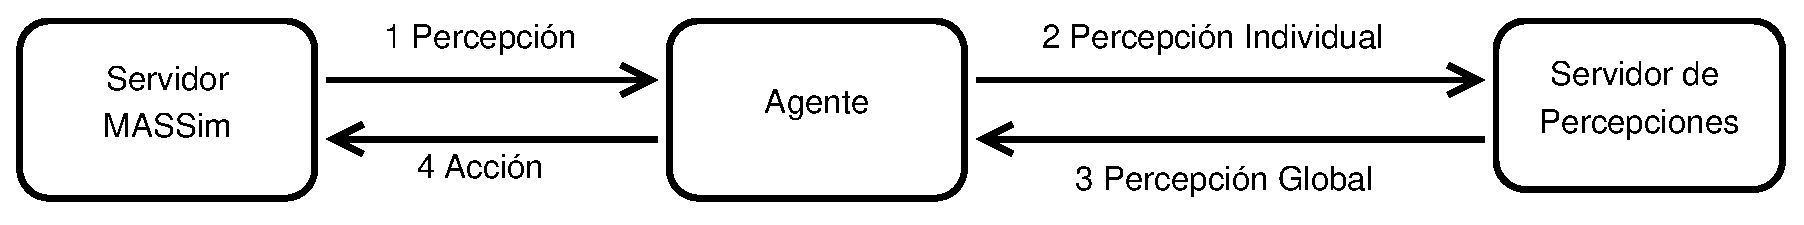
\includegraphics[scale=.5]{graficos/eps/system_architecture.eps}
 \caption{Diagrama de la secuencia de acciones de cada ciclo de la simulación.}
 \label{fig:system_architecture}
 \end{figure}

%---------------------------------------------CONEXION MASSIM-SERVER-%
\section[Conexión con el MASSim Server]
 {Conexión del Agente con el Servidor MASSim}
 \label{sec:conexion_massim}

 El protocolo de comunicación con el servidor MASSim especificado por 
 el enunciado del concurso MAPC define que los agentes y el servidor 
 intercambian mensajes en formato XML codificados por UTF-8, con un 
 byte nulo para indicar el final del mensaje. 

%--------------------------------------------PROTOCOLO MASSIM-SERVER-%
\subsection[Protocolo del MASSim Server]
 {Protocolo de comunicación con el servidor MASSim}
 \label{sub:protocolo_massim}

 Los agentes de cada equipo se ejecuta localmente, mientras que el entorno
 simulado, sobre el cual los agentes de todos los equipos realizan acciones,
 corria en un servidor remoto.

 Los agentes se comunican con el servidor del concurso a traves de un socket TCP/IP estandard con una interface de socket, sobre el cual intercambiaban mensajes XML.
 Los mensajes son documentos bien formados de XML, los mensajes mal formados son ignorados por el servidor de simulación. 

 Cada torneo consiste de un numero de partidos.
 Una partido es una secuencia de simulaciones en las cuales varios equipos de agentes compiten en varios escenarios del entorno.
 Desde el punto de vista del agente, el torneo consiste de una secuencia de simulaciones, en distintos escenarios, contra distintos equipos.

 El torneo se divide en tres fases:

 \begin{enumerate}
 \item La fase inicial,
 \item la fase de simulación,
 \item la fase final.
 \end{enumerate}

 Durante la fase inicial, los agentes se conectan al servidor de simulación y se identifican mediante un nombre y una contraseña (mensaje \texttt{AUTH-REQUEST}) que puede resultar en exito o fracaso.
 Luego de una autentificación exitosa, los agentes deberán esperar a que comienze la primera simulación del torneo.
 La figura \ref{fig:fase_inicial} muestra la fase inicial.

 \textbf{
 \begin{tabular}{|l|}
 \hline
 FIGURA DE FASE INICIAL \\
 \hline
 \end{tabular}
 }

 En cada paso de la simulación el agente recibe una percepción de s u  entorno (mensaje \texttt{REQUEST-ACTION}) y debe responder con la  acción (mensaje \texttt{ACTION}).
 El agente debe entregar su respuesta antes de un tiempo determinado.
 El mensaje de la acción debe contener el identificador de la acción y  sus parametros. 
 La figura \ref{fig:fase_simulacion} muestra la fase de simulación. 

 \textbf{
 \begin{tabular}{|l|}
 \hline
 FIGURA DE FASE SIMULACION \\
 \hline
 \end{tabular}
 }

 Cuando la simulación concluye, los agentes participantes reciben una notificación de su conclusión (mensaje \texttt{SIM-END}) que incluye el resultado de la simulación. 
 Todo agente que actualmente no participa en una simulación debe esperar hasta que el servidor de simulación les notifique que o bien comienza una simulación o que el torneo concluye. 

 Al final del torneo, todos los agentes reciben una notificación (mensaje \texttt{BYE}) y a continuación el servidor de simulación cerrará las conexiones a los agentes
 La figura \ref{fig:fase_final} muestra la fase final. 

 \textbf{
 \begin{tabular}{|l|}
 \hline
 FIGURA DE FASE FINAL \\
 \hline
 \end{tabular}
 }

 \subsubsection{Reconexión}
 \label{sub:reconexion_massim} 

 Si un agente pierde su conexión con el servidor de simulación, el torneo continúa sin interrupción, y las acciones del agente desconectado se consideran vacias (de tipo \texttt{skip}). 
 Los agentes son responsables de mantener la conexión al servidor de simulación y en el caso de una interrupción, se les permite reconectarse.
 Los agentes se reconectan realizando la misma secuencia de pasos que al principio del torneo.
 Después de establecer la conexión con el servidor de simulación, envia un mensaje \texttt{AUTH-REQUEST} y recibe un \texttt{AUTH-RESPONSE}. 
 Luego de una autentificación exitosa, el servidor envia un mensaje \texttt{SIM-START} al agente. 
 Si el agente participa en una simulación que esta corriendo, el mensaje \texttt{SIM-START} se envia inmediatamente después del mensaje \texttt{AUTH-RESPONSE}.
 De lo contrario el agente esperará hasta que comienze la próxima simulación en la cual participa.
 En el siguiente paso cuando el agente debe seleccionar una acción, recibe un mensaje \texttt{REQUEST-ACTION} estandard conteniendo la percepción del agente ese turno y la simulación procede de manera normal.
 La figura \ref{fig:reconexion_massim} muestra el protocolo de reconexión. 

%---------------------------------------------------FORMATO MENSAJES-%
\subsection{Formato de mensajes}
 \label{sub:formato_mensajes}

 \textbf{
 \begin{tabular}{|l|}
 \hline
 TODO : entro en detalle con la descripcion de los mensajes? \\
 \hline
 \end{tabular}
 }

\subsubsection{\texttt{AUTH-REQUEST}}

\subsubsection{\texttt{AUTH-RESPONSE}}

\subsubsection{\texttt{SIM-START}}

\subsubsection{\texttt{SIM-END}}

\subsubsection{\texttt{BYE}}

\subsubsection{\texttt{REQUEST-ACTION}}

\subsubsection{\texttt{ACTION}}

  \begin{verbatim}
  <?xml version="1.0" encoding="UTF-8" standalone="no"?>
    <message type="action">
      <action id=\"ID\" type=\"TYPE\"/>
    </message>\0
  \end{verbatim}
  
  En el caso de las acciones que requieren un parámetro adicional, la
  representación es:
  
  \begin{verbatim}
  <?xml version="1.0" encoding="UTF-8" standalone="no"?>
    <message type="action">
      <action id="ID" param="PARAM" type="TYPE"/>
    </message>\0
  \end{verbatim}
  
  donde {\tt ID} es el identificador de mensaje enviado por el servidor
  MASSim en la percepcion, {\tt TYPE} es el tipo de acción y {\tt PARAM}
  es el parametro. 
  
  {\tt TYPE} puede ser uno de:
  
  \begin{itemize}
  \item \tt{skip}
  \item \tt{goto}
  \item \tt{attack}
  \item \tt{parry}
  \item \tt{probe}
  \item \tt{survey}
  \item \tt{inspect}
  \item \tt{repair}
  \item \tt{recharge}
  \item \tt{buy}
  \end{itemize}

%---------------------------------------------------------ARQ AGENTE-%
\section{Arquitectura del agente}
 \label{sec:arquitectura_agente}

 Esta sección tiene el objetivo de analizar el diseño y estructura de 
 un agente individual.

%-------------------------------------------------------------DISEÑO-%
\subsection{Diseño general}
 \label{sub:diseno_general}
 
 % ORIGEN: marcov 
 El programa agente presenta una estructura simple en cuanto a su
 división.
 La interacción con el entorno y el procesamiento inicial de la
 información recibida finalizan con la generación de una serie de
 creencias que son incorporadas a la base de conocimiento mantenida por
 el agente.
 Este conjunto de creencias es empleado posteriormente por el módulo
 encargado de tomar decisiones.
 La forma en que se estructuran los componentes principales es
 detallada a continuación.

 % ORIGEN: report
 El agente parsea las opciones pasadas por linea de comando al iniciar 
 que determinaran sus paremetros de comportamiento.
 Entre ellos estan los detalles de autentificación que utilizará con 
 el MASSim server (nombre de usuario y contraseña), si esta habilitado 
 el registro de eventos y su nivel de verbosidad, la ubicación en la 
 red del Servidor de Percepciones, y si el agente operará en modo 
 ``dummy'' (en el cual no utiliza argumentación en el proceso 
 deliberativo) o no. 

 % ORIGEN: report
 El mensaje de inicio de simulación es enviado por el MASSim server 
 cada vez que un agente se conecta.  
 
 Los posibles tipos de mensajes son \texttt{sim-start}, \texttt{sim-end}, 
 \texttt{request-action} y \texttt{bye}. 

 Para cada solicitud de acción, la cual incluye la percepción del 
 agente para ese turno, el agente procesará el mensaje, enviando la 
 información que desea compartir con los demás agentes del equipo al 
 servidor de Percepciones, reincorporá la respuesta del 
 Servidor de Percepciones a su base de conocimiento, iniciará el 
 proceso deliberativo para llegar a una decisión sobre cual acción 
 tomar, y finalmente enviará un mensaje representando su decisión al 
 servidor MASSim.   

\subsubsection{Estructura básica del agente}
 \label{subsub:estructura_basica_de_agente}
  
 El programa principal del agente es el encargado de manejar la
 comunicación con los servidores, tanto el del juego como el de
 percepciones (presentado a continuación).
 También es responsable de parsear y procesar la información contenida
 en la percepción para darle el formato interpretado por la base de
 conocimientos, y enviar la acción que ha sido elegida por el módulo
 de toma de decisiones.
 
 \begin{figure}
 \centering
 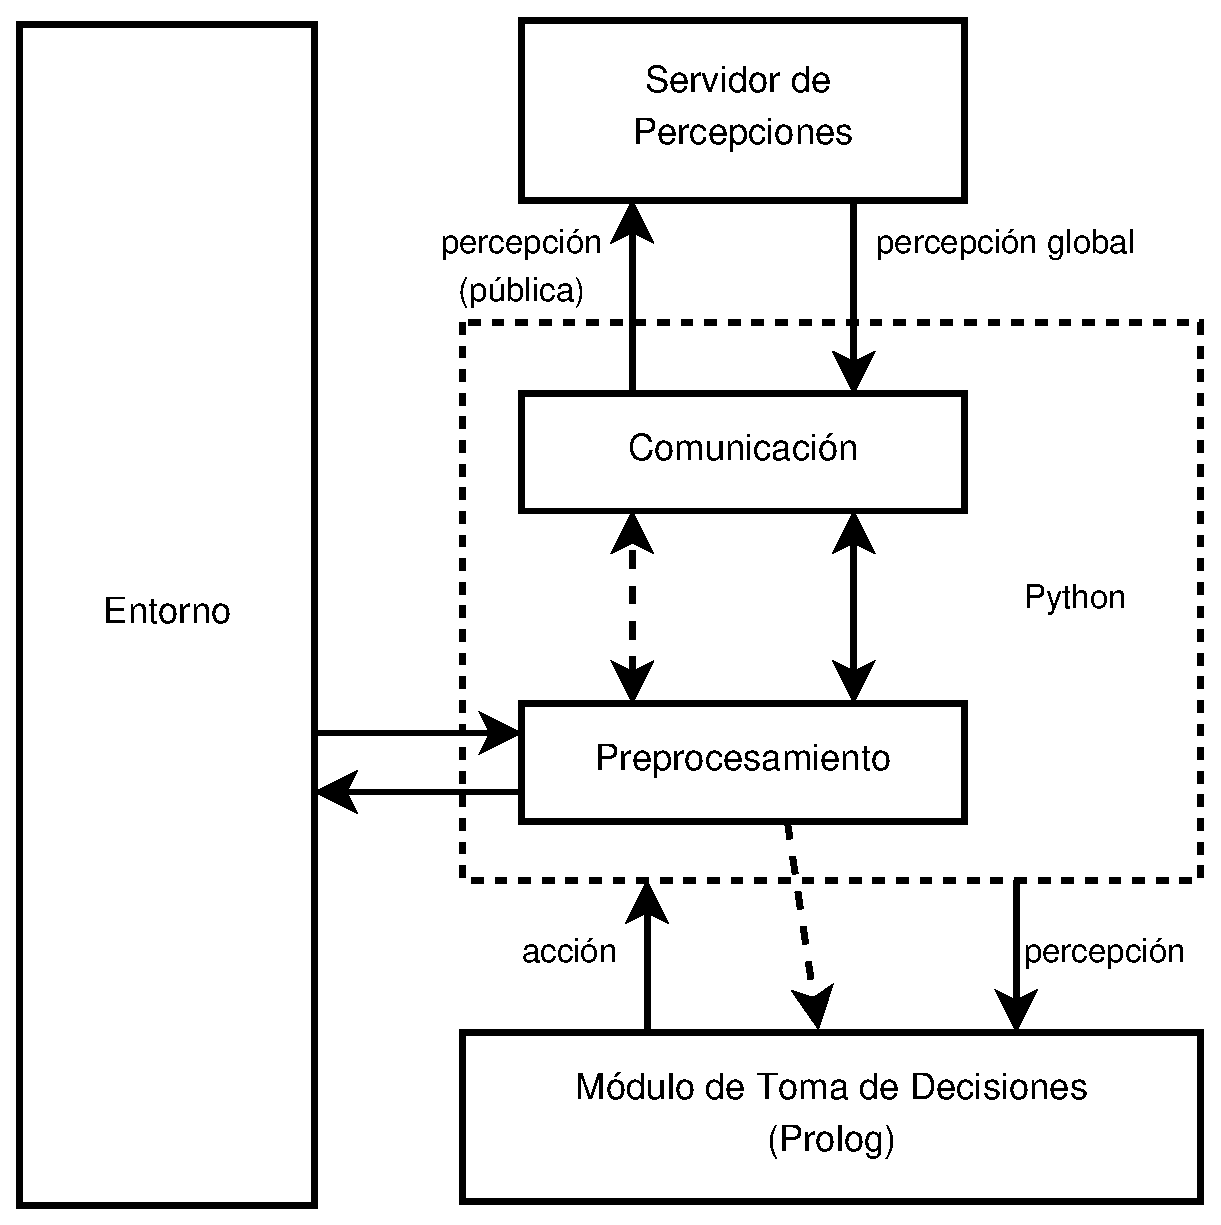
\includegraphics[scale=.4]{graficos/eps/agent_architecture.eps}
 \caption{Diagrama de la arquitectura del agente. Las líneas punteadas
 representan el flujo de control, y las líneas contínuas representan el
 flujo de datos.}
 \label{fig:architecture}
 \end{figure}
 
 El servidor de percepciones (SP) es un programa independiente,
 encargado de unificar las percepciones de todos los agentes que se
 encuentran en ejecución.
 Recibe sus percepciones individuales y retorna a cada uno de ellos el
 conjunto de datos que aún no poseen, de manera que todos los agentes
 del equipo cuenten con la misma información en cuanto al estado del
 escenario.
  
 En cada iteración de la simulación, el agente recibe un mensaje por
 parte del servidor del juego, el cual contiene la información
 asociada a la percepción del turno en disputa.
 Este mensaje es parseado y traducido en una estructura que permite
 manipular los datos con mayor facilidad.
 Los datos son divididos en dos conjuntos, uno ``público'', el cual es
 compartido con los demás agentes del equipo, y uno ``privado''.
 La sección pública de datos es compartida a través del mencionado
 servidor de percepciones.
 
 El agente une entonces su propia percepción con la percepción global
 recibida del servidor de percepciones, y genera un único conjunto de
 datos.
 Esta información es incorporada a la base de conocimientos,
 estableciendo nuevas creencias para el agente.
 
 El módulo de toma de decisiones, analizado en la sección
 \ref{sec:arquitectura_bdi}, es el que implementa el modelo BDI
 respetado por el agente.
 Este módulo es consultado en cada iteración para obtener la próxima
 acción a ser ejecutada.
 Una vez que el flujo de control retorna al programa principal, la
 acción seleccionada es enviada al servidor del juego.
  
\subsubsection{BASE DE CONOCIMIENTO}

\subsection{ARQUITECTURA BDI}

\subsection{ARGUMENTACION}

\subsection{PLANIFICACION}

\subsection{EJECUCION}

 
\clearemptydoublepage


\chapter{Servidor de Percepciones}
\label{chap:servidor_de_percepciones}

\begin{verbatim}
[ ] capa de conexion con el servidor massim
[ ] formato de los mensajes percepciones/acciones
[ ] esquema de codificacion de las percepciones para mandar al PS (estructura y cpickle)
[ ] protocolo de comunicacion con el PS
[ ] esquema de reconexion para agentes caidos
[ ] algoritmo del PS
\end{verbatim}

\section{Conexión del Agente con el Servidor MASSim}

El protocolo de comunicación con el servidor MASSim especificado por 
el enunciado del concurso MAPC define que los agentes y el servidor 
intercambian mensajes en formato XML codificados por UTF-8, con un 
byte nulo para indicar el final del mensaje. 

\subsection{Protocolo de comunicación con el servidor MASSim}

TODO

\subsection{Formato de mensajes}

TODO

\subsubsection{Percepciones}

TODO

\subsubsection{Acciones}

  Las acciones se representan con la cadena de caracteres:
  
  \begin{verbatim}
  <?xml version="1.0" encoding="UTF-8" standalone="no"?>
    <message type="action">
      <action id=\"ID\" type=\"TYPE\"/>
    </message>\0
  \end{verbatim}
  
  En el caso de las acciones que requieren un parámetro adicional, la
  representación es:
  
  \begin{verbatim}
  <?xml version="1.0" encoding="UTF-8" standalone="no"?>
    <message type="action">
      <action id="ID" param="PARAM" type="TYPE"/>
    </message>\0
  \end{verbatim}
  
  donde {\tt ID} es el identificador de mensaje enviado por el servidor
  MASSim en la percepcion, {\tt TYPE} es el tipo de accion y {\tt PARAM}
  es el parametro. 
  
  {\tt TYPE} puede ser uno de:
  
  \begin{itemize}
  \item \tt{skip}
  \item \tt{goto}
  \item \tt{attack}
  \item \tt{parry}
  \item \tt{probe}
  \item \tt{survey}
  \item \tt{inspect}
  \item \tt{repair}
  \item \tt{recharge}
  \item \tt{buy}
  \end{itemize}

\section{Conexión del Agente con el Servidor de Percepciones}

TODO

\section{Formato de Percepciones}

TODO

\section{Protocolo de Comunicación con el Servidor de Percepciones}

TODO

\section{Esquema de Codificación}

 Tras la recepción de la percepción del servidor, el parseo del XML y
 su transformación en diccionarios nativos de Python, el agente
 retransmite la informacion recibida al servidor de percepciones.
 Aunque es factible enviar la percepcón en formato XML o como la
 representación de la estructura de datos en memoria del agente, unos
 de los objetivos es distribuir tanto como posible el trabajo realizado
 por el sistema.
 Como las tareas principales realizadas por el servidor de percepciones 
 son la union de la información y la diferencia de cada percepción 
 individual con el total, se implemento un esquema más de codificacion. 
 Se transforma el diccionario que contiene la percepción en una 
 estructura sobre la cual se pueden realizar operaciones de conjunto de 
 manera eficiente. 
 
TODO

\subsection{Esquema de Reconexión para Agentes Caidos}

Si el agente pierde la conexión, o 
 
\clearemptydoublepage

\begin{thebibliography}{99}
\addcontentsline{toc}{chapter}{Bibliografía}
\bibitem{jade99}
  F. Bellifemine, A. Poggi, G. Rimassa,
  \emph{JADE - A FIPA-compliant agent framework}.
  CSELT internal technical report,
  1999.
\bibitem{dev01}
  F. Bellifemine, A. Poggi, G. Rimassa,
  \emph{Developing multi-agent systems with a FIPA-compliant agent framework}.
  Software - Practice And Experience,
  2001.
\bibitem{coord00}
  R. S. Cost, Y. Labrou, T. Finin,
  \emph{Coordinating Agents using Agent Communication Languages Conversations}.
  2000. 	
\bibitem{apl03}
  Dastani et al.,
  \emph{A Programming Language for Cognitive Agents: Goal Directed 3APL}.
  Proceedings of the First Workshop on Programming Multiagent Systems: Languages, frameworks, techniques, and tools,
  2003.
\bibitem{coop96}
  Doran et al.,
  \emph{On Cooperation in Multi-Agent Systems. The Knowledge Engineering Review}.
  1996.
\bibitem{delp04}
  A. J. García, G. R. Simari,
  \emph{Defeasible logic programming: An argumentative approach}.
  Journal of Theory and Practice of Logic Programming,
  2004.
\bibitem{int05}
  A. J. García, M. Tucat, G. R. Simari,
  \emph{Interaction Primitives for Implementing Multi-agent Systems}.
  Interaction Primitives for Implementing Multi-agent Systems,
  2005.
\bibitem{mult99}
  M. Huhns, L. Stephens,
  \emph{Multiagent Systems and Societies of Agents}.
  Multiagent Systems: A Modern Approach to Distributed Artificial Intelligence,
  1999.
\bibitem{arg98}
  N. R. Jennings et al.,
  \emph{Argumentation-Based Negotiation}.
  Proceedings of the International Workshop on Multi-Agent Systems,
  1998.
\bibitem{soc99}
  S. Kalenka, N. R. Jennings,
  \emph{Socially Responsible Decision Making by Autonomous Agents}.
  Proceedings of the 5th International Colloquium on Cognitive Science,
  1999.
\bibitem{neg96}
  J. Müller,
  \emph{Negotiation Principles}.
  Foundations of Distributed Artificial Intelligence,
  1996.
\bibitem{mod91}
  A. Rao, M. Georgeff,
  \emph{Modeling rational agents within a BDI-architecture}.
  Proceedings of the Second International Conference on Principles of Knowledge Representation and Reasoning,
  1991.
\bibitem{bdi95}
  A. S. Rao, M. P. Georgeff,
  \emph{BDI Agents: From Theory to Practice}.
  Proceedings of the First International Conference on Multi-Agent Systems,
  1995.
\bibitem{arg02}
  S. V. Rueda, A. J. García, G. R. Simari,
  \emph{Argument-based Negotiation among BDI Agents}.
  Journal of Computer Science and Technology,
  2002.
\bibitem{ia99}
  M. Wooldridge,
  \emph{Intelligent Agents}.
  Multiagent Systems, The MIT Press,
  1999.
\bibitem{brat99}
    M. E. Bratman,
    \emph{Intention, Plans, and Practical Reason}.
    Cambridge University Press,
    1999.
\bibitem{searle1985}
	J.R. Searle,
  \emph{Intentionality, an Essay in the Philosophy of Mind}.
  Cambridge University Press,
  1983.

\end{thebibliography} 
\clearemptydoublepage

\bibliographystyle{thesis} % archivo Thesis.bst creado por Alejandro Stankevicius (UNS)
\bibliography{tesina}      % indica de donde sacar la informaci�n para crear doc.bbl

\end{document}
